\documentclass[NET,a4,12pt,english]{netforms}

\usepackage[utf8]{inputenc}
\usepackage{tumlang}
\usepackage{tumcontact}
\usepackage{scrpage2}
\usepackage{pgfgantt}
\usepackage{graphicx}
\usepackage{tikz}
\usetikzlibrary{backgrounds,calc,shadings,shapes.arrows,shapes.symbols,shadows}
\pgfkeys{/pgf/.cd,
  parallelepiped offset x/.initial=2mm,
  parallelepiped offset y/.initial=2mm
}
\geometry{%
	top=10mm,
	bottom=10mm,
	left=25mm,
	right=25mm,
	headsep=1.5cm,
	includehead,
}

% Alle Konfigurationsbefehle sind optional. Fehlende Befehle fueheren einfach
% zu "blank forms".

% Typ der Arbeit/Einstellung. Gueltige Argumente sind:
% bachelor,master,diplom,idp,gr,hiwi,other
% Falls 'other' gewaehlt wird, kann als optionales Argument eine spezielle Art
% von Abschlussarbeit angegeben werden, z.B. \type[Sklave]{other}. Andernfalls
% wird 'Other' als Standardbeschreibung gesetzt.
\type{bachelor}

% Informationen ueber den Studenten. Sollte selbsterklaerend sein.
\anrede{Herr}
\nachname{Nguyen}
\vorname{Huu Tung}
\matrikel{03682804}
\sunhalle{sunaccount}
\semester{7}{WiSe\,2019}
\studientelefon{}{0174 2758818}
\heimattelefon{}{--}
\studienadresse{Admiralbogen 28}{80939 M\"unchen}
\heimatadresse[adresszusatz=,appartment=]{}{}
\mail{nguyenhu@tum.de}

% Informationen ueber die Arbeit. Sollte selbsterklaerend sein.
\themensteller{\NEThead}
\beginn{12}{2019}
\endt{04}{2020}
\betreuer{Simon Bauer, Benedikt Jaeger}
\title{Available Bandwidth Estimation}{Verf\"ugbare Bandbreitenabsch\"atzung}
\studiengang{Informatik}


% Falls \type{hiwi} gesetzt wurde, wird die Taetigkeit auf dem Aufnahmeformular
% des Lehrstuhls angegeben.
\taetigkeit{test}



\pagestyle{scrheadings}
\clearscrheadfoot
\chead{\TUMheader{1cm}}

\renewcommand{\maketitle}{%
	\begin{center}
		\textbf{\introductoryheadline}%

		\Large%
		\textbf{\thetitle}%
	\end{center}

	\footnotesize%
	\hrule
	\vskip1ex
	\begin{tabular}{ll}
		\thenamelabel: & \thevorname{} \textbf{\thenachname}\\
		\theadvisorlabel: & \hspace*{-.5ex}\thebetreuer\\
		\thesupervisorlabel: & \chairhead\\
		\thebeginlabel: & \thebeginnmonat/\thebeginnjahr\\
		\theendlabel: & \theendmonat/\theendjahr\\
	\end{tabular}
	\vskip1ex
	\hrule
	\vskip4ex
}

\linespread{1.2}
\setlength{\parskip}{.5\baselineskip}

\begin{document}
\maketitle

\section*{Topic}
Observing the rapid development in technology such as realtime systems or the popularity of streaming services, the Internet's penetration rate increased tenfold in the last 20 years \cite{lin1973}.% https://www.internetworldstats.com/stats.htm // More Example such as streaming popular more use of realtime systems 
Thus, it is essential to have knowledge about the available bandwidth to enhance quality-of-service (QoS) requirements by selecting the optimal route for a designated service. As a consequence, there are several end-to-end tools for available-bandwidth estimation such as Pathload \cite{pathload}. Since most tools require access at both ends, their applicability is limited. Additionally, they rely on UDP/ICMP which is often blocked or rate limited \cite{proceedings:passivactivemeas} .% Cite abget 
Of more interest are single-ended tools based on TCP such as abget \cite{proceedings:passivactivemeas}, ABwprobe \cite{abwprobe} and its successor fabprobe \cite{fabprobe}. Their ideas are based on Pathload's \cite{pathload} approach and redesigned for estimation with TCP. As a result of TCP, it is more complicated to estimate the available-bandwidth because packets can take different routes from host to host. Although the source code is available, it is not possible to run the code today. Therefore the goal of this thesis is to implement a single-end available bandwidth estimation tool based on the fabprobe and abget, evaluate its accuracy and applicability for large-scale Internet measurements. \\
\\
Following research questions are to be considered:

\begin{enumerate}
	\item How good is the performance?
	\item Trade-off between accuracy and efficiency?
	\item What limitations and restrictions constraint the usage on the internet?
\end{enumerate} 

\section*{Basic Ideas}

One approach to this problem is Abget an iterative algorithm, based on the idea of pathload which transmits periodic TCP instead of UDP packet streams. In order to send packets at a certain rate R the client sends "fake" ACKs over to the TCP server, through a raw IP socket interface to emulate the TCP protocol \cite{proceedings:passivactivemeas} .
Because of this, it is possible to determine the available-bandwidth through an increasing or decreasing trend in the One-Way-Delay (OWD). This implies the probing rate R is higher or lower than the available-bandwidth.

An alternative to solve the problem is fabprobe, that uses a binary search-like algorithm \cite{fabprobe}. % ABWprobe mehr einbeziehen um auf related work zu verweisen
First the path is probed with a fleet of packets at an initial rate R. The available-bandwidth can be derived from the packet's RTT. If the RTT shows an increasing trend, the rate R is reduced, thus meaning the rate is greater than the available-bandwidth. Consequently, a decreasing trend results in increasing R. Fabprobe's main focus is the trade-off between efficiency and accuracy, with fewer numbers of samples to achieve the highest accuracy possible.

\section*{Approach}
Since fabprobe is designed for large-scale measurement, we will focus on its approach. First, the tool will be implemented and tested in Mininet \cite{mininet}, a small testbed, under control.
% Test aufbau genauer erklären
The results will be evaluated according to accuracy, stability, overhead, mean relative error and derivation. If the results are promising, a test on the Internet will follow and be tested against an active end-to-end tool such as pathload to verify the previous results. 
\begin{center}
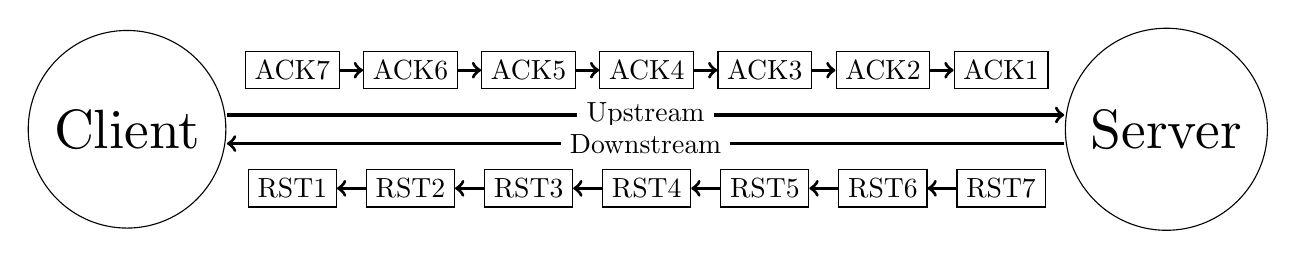
\begin{tikzpicture}[scale = 3.0]
	\tikzstyle{vertex} = [circle, draw=black, scale = 2.0]
	\tikzstyle{rect} = [rectangle, draw=black]
	\tikzstyle{edge} = [->, very thick]
	\node[vertex](client) at (-0.2,0){Client};
	\node[vertex](server) at (4.2,0){Server};
	\node[rect](ACK7) at (0.5,0.25){ACK7};
	\node[rect](ACK6) at (1,0.25){ACK6};
	\node[rect](ACK5) at (1.5,0.25){ACK5};
	\node[rect](ACK4) at (2,0.25){ACK4};
	\node[rect](ACK3) at (2.5,0.25){ACK3};
	\node[rect](ACK2) at (3,0.25){ACK2};
	\node[rect](ACK1) at (3.5,0 .25){ACK1};
	\node[rect](RST1) at (0.5,-0.25){RST1};
	\node[rect](RST2) at (1,-0.25){RST2};
	\node[rect](RST3) at (1.5,-0.25){RST3};
	\node[rect](RST4) at (2,-0.25){RST4};
	\node[rect](RST5) at (2.5,-0.25){RST5};
	\node[rect](RST6) at (3,-0.25){RST6};
	\node[rect](RST7) at (3.5,-0.25){RST7};
	\draw[edge] ([yshift=0.4ex]client.east) -- ([yshift=0.4ex]server.west) node [midway, fill= white]{Upstream};
	\draw[edge] ([yshift=-0.4ex]server.west) -- ([yshift=-0.4ex]client.east) node [midway, fill=white]{Downstream};
	\draw[edge](ACK7) -- (ACK6);
	\draw[edge](ACK6) -- (ACK5);
	\draw[edge](ACK5) -- (ACK4);
	\draw[edge](ACK4) -- (ACK3);
	\draw[edge](ACK3) -- (ACK2);
	\draw[edge](ACK2) -- (ACK1);
	\draw[edge](RST7) -- (RST6);
	\draw[edge](RST6) -- (RST5);
	\draw[edge](RST5) -- (RST4);
	\draw[edge](RST4) -- (RST3);
	\draw[edge](RST3) -- (RST2);
	\draw[edge](RST2) -- (RST1);
\end{tikzpicture}
\end{center}
\section*{Schedule}

\resizebox{\textwidth}{!}{
\begin{ganttchart}[hgrid, vgrid={dotted}, group label font={\bf}, x unit=7mm, bar/.append group/.append style={draw=black}]{1}{20}
\gantttitle[y unit title = 1.7 cm]{December}{4}
\gantttitle[y unit title = 1.7 cm]{January}{4}
\gantttitle[y unit title = 1.7 cm]{February}{4}
\gantttitle[y unit title = 1.7 cm]{March}{4}
\gantttitle[y unit title = 1.7 cm]{April}{4}\\

\ganttbar{Analysis}{1}{4}\\
\ganttbar{Implementation}{3}{14}\\
\ganttbar{Testbed setup}{7}{16}\\
\ganttbar{Testing and Validation}{8}{16}\\
\ganttbar{Thesis writing}{9}{18}]
\end{ganttchart}
} %

\bibliographystyle{IEEEtran}
\bibliography{IEEEabrv,lit}

\end{document}
